\documentclass[11pt, oneside]{article}   	
\usepackage[margin=1in]{geometry}                		
\geometry{letterpaper}                   		
\usepackage{graphicx}						
\usepackage{amssymb}
\usepackage{amsmath}
\usepackage{amsthm}
\usepackage{enumerate}
\graphicspath{ {./hw4pic/} }


%Commands above this line set up the type of document, and ensure it has access to the LaTeX files needed to understand your commands.

%Here, I define some "shortcuts" for notation I commonly use. 
\newcommand{\N}{\mathbb N}
\newcommand{\Z}{\mathbb Z}
\newcommand{\Q}{\mathbb Q}
\newcommand{\C}{\mathbb C}
\newcommand{\R}{\mathbb R}
\newcommand{\F}{\mathbb F}

\newtheorem*{proposition}{Proposition}
\newtheorem*{theorem}{Theorem}

\title{Homework 1}
\author{The Author} 
%\date{}			




%THIS IS WHERE THE ACTUAL TEXT OF THE DOCUMENT BEGINS.				
\begin{document}

\begin{center}\noindent{\bf Math 381:  Homework \#4}\\Mingchen Li\\ \end{center}

\begin{enumerate}
    \item[Problem 1] 
    \begin{enumerate}
        \item $X \sim Bin(n, p)$ when p = 1/2, n = 5, 10, 20.

        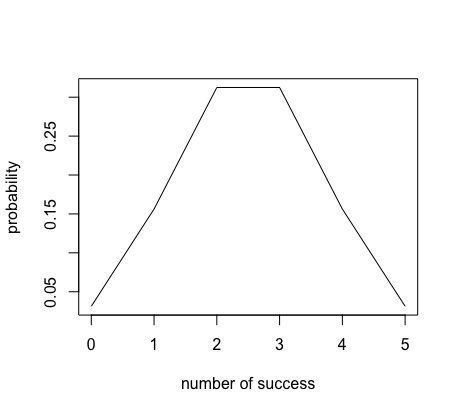
\includegraphics[scale=0.3]{111}
        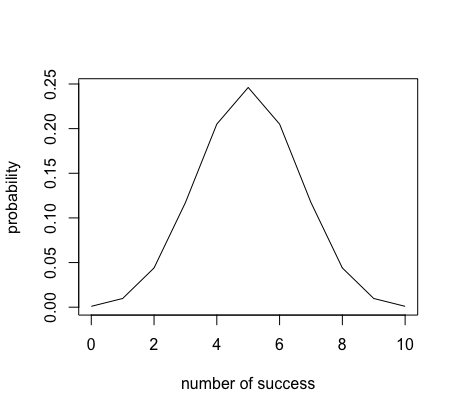
\includegraphics[scale=0.3]{112}
        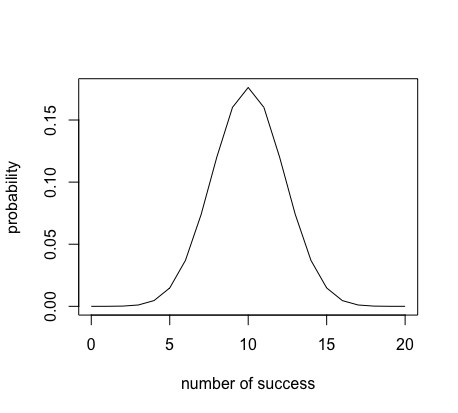
\includegraphics[scale=0.3]{113}

        
        \item $X \sim Bin(n, p)$ when p = 1/10, n = 5, 10, 20.
        
        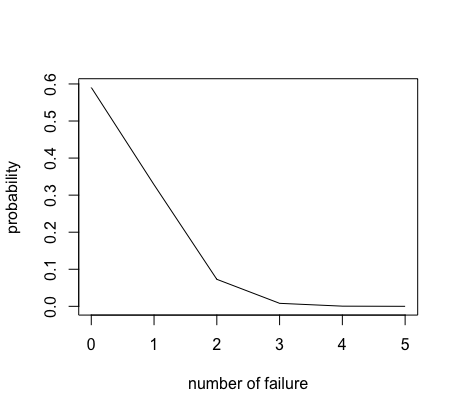
\includegraphics[scale=0.3]{121}
        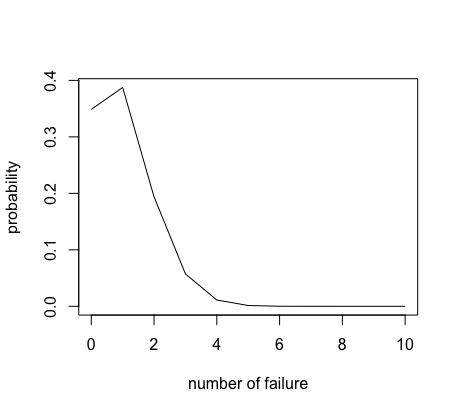
\includegraphics[scale=0.3]{122}
        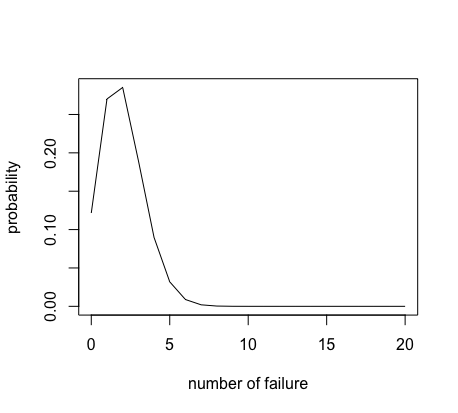
\includegraphics[scale=0.3]{123}
        
        \item $X \sim Geom(p)$ when p = 1/2
        
        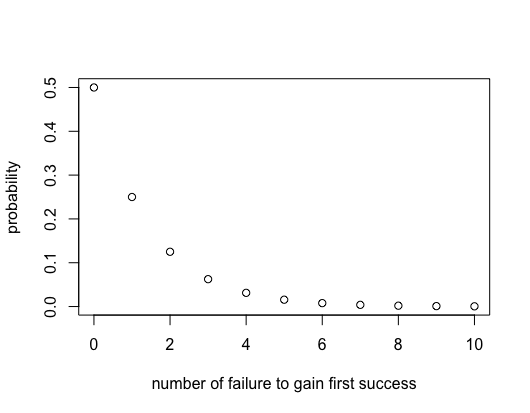
\includegraphics[scale=0.3]{131}
        \item $X \sim$ Hypergeom(15, 6, 3)
        
        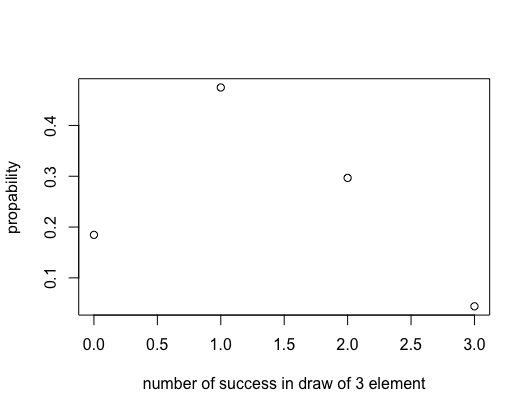
\includegraphics[scale =0.3]{141}
    \end{enumerate}
    
    \newpage
    \item[Problem 2]
    \begin{enumerate}
        \item $X \sim Bin(n, p)$ when p = 1/2, n = 5, 10, 20.

        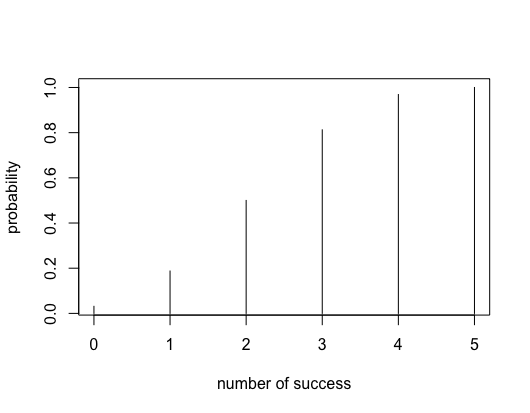
\includegraphics[scale=0.3]{211}
        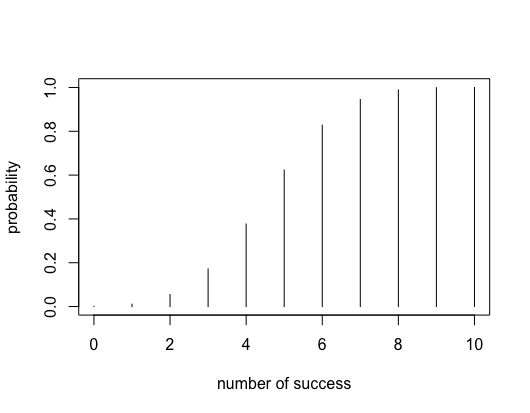
\includegraphics[scale=0.3]{212}
        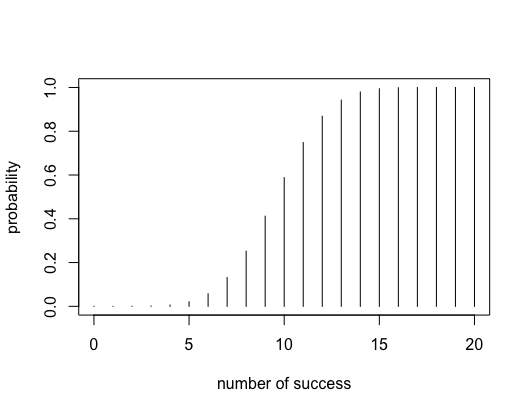
\includegraphics[scale=0.3]{213}
        
        \item $X \sim Bin(n, p)$ when p = 1/10, n = 5, 10, 20.
        
        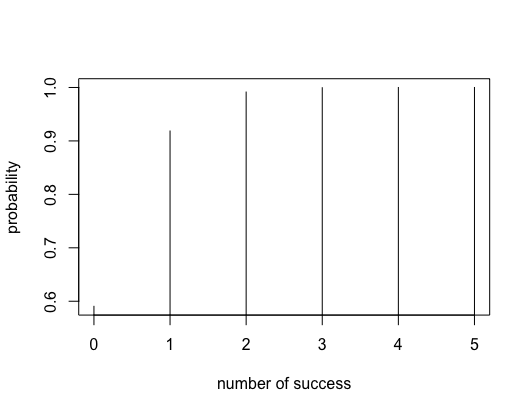
\includegraphics[scale=0.3]{221}
        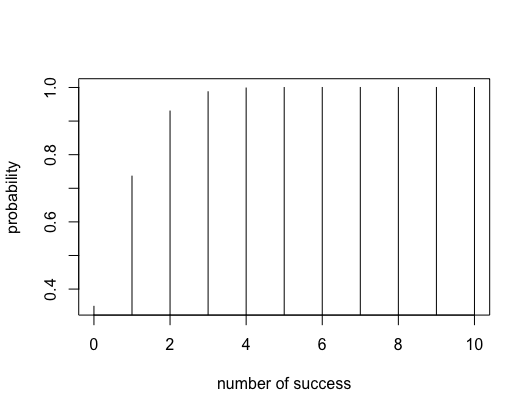
\includegraphics[scale=0.3]{222}
        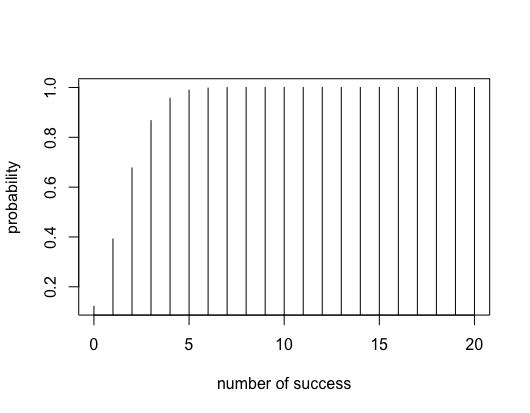
\includegraphics[scale=0.3]{223}
        \item $X \sim Geom(p)$ when p = 1/2
        
        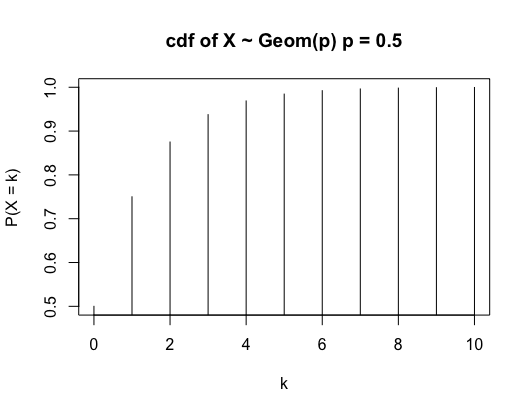
\includegraphics[scale=0.3]{231}
        \item $X \sim$ Hypergeom(15, 6, 3)
        
        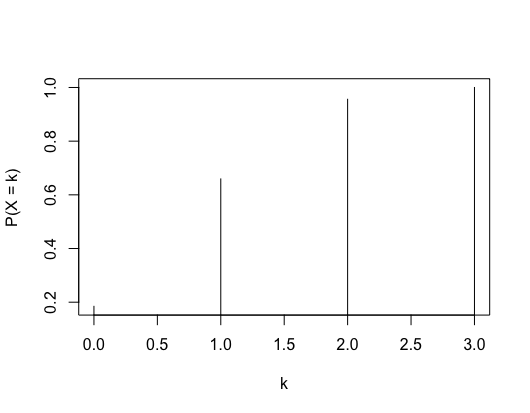
\includegraphics[scale =0.3]{241}
    \end{enumerate}
    
    \newpage
    \item[Problem 3] 
    \begin{enumerate}

        \item 2.21 :
            Jane must get at least three of the four problems on the exam correct to get an A. She has been able to do 80 $\% $ of the problems on old exams, so she assumes that the probability she gets any problem correct is 0.8. She also assumes that the results on different problems are independent.
            \begin{enumerate}
                \item What is the probability she gets an A?
                \begin{proof}
                P(Jane gets A)= P(Jane answer 3 question correctly) +P(Jane answer 4 question correctly)= ${4\choose 3}\times 0.8^3\times 0.2+{4\choose 4}\times 0.8^4$=0.8192
                \end{proof}
                \item If she gets the first problem correct, what is the probability she gets an A?
                \begin{proof}
                P(Jane gets A $|$ Jane gets first problem correct) = P(Jane get 2 question correct within the 3 remaining questions)+P(Jane get 3 question correct within the 3 remaining questions)= ${3\choose 2}\times 0.8^2\times 0.2+{4\choose 4}\times 0.8^3=0.896$
                \end{proof}
            \end{enumerate}
        
        \item 2.24:
        A team of three is chosen randomly from an office with 2 men and 4 women. Let X be the number of women on the team.
        
        \begin{enumerate}
            \item Identify the probability distribution of X by name.
            
            It is a Hyper Geometric distribution. $X\sim Hypergeom(6, 4,3)$
            
            \item Give the probability mass function of X.
            
            P(X=0)=P(there are 0 female in the sample of 3)=0
            
            P(X=1)=P(there are 1 female in the sample of 3)=$\dfrac{{4\choose  1 } {2  \choose 2}}{{6\choose 3}}$ = 0.2
            
            P(X=2)=$\dfrac{{4\choose  2 } {2  \choose 1}}{{6\choose 3}}$ = 0.6
            
            P(X=3)=$\dfrac{{4\choose  3 } {2  \choose 0}}{{6\choose 3}}$ = 0.2
            
            \end{enumerate}
        \end{enumerate}
    
    
    \item [Problem 4]
    (2.35) We shuffle a deck of cards and deal two cards. Find the
    probability that the first card is a queen and the second is a spade.
    \begin{proof}
    Since the card is uniformly random drawn, we shall denote P(A,B) as P(first draw is A $\cap$ second draw is B). Since each draw is independent, $P(AB)=P(A)P(B)$
    
    P(Queen, spade)=P(Spade Queen, Spade) + P(non-Spade Queen, Spade)=$1/54 \times 12/53 + 3/54\times 13/53= 51/2862\approx 0.018$
    \end{proof}
    \item [Problem 5]
    (2.41) Two factories I and II produce phones for brand ABC. Factory I produces 60$\%$ of all ABC phones, and factory II produces 40\%. 10\% of phones produced by factory I are defective, and 20\% of those produced by factory II are defective. You purchase a brand ABC phone, and assume this phone is randomly chosen from all ABC phones. Suppose the phone is not defective. What is the probability that it came from factory II?
    \begin{proof}
    Since the phone is randomly chosen
    \begin{enumerate}
        \item P(Come from A)=0.6
        \item P(Come from B)=0.4
        \item P(not defective $|$ Come from A)=0.9
        \item P(not defective $|$ Come from B)=0.2.
    \end{enumerate}
    
   By Bayes theorem: P(Come from B$|$not defective)=
   \[\dfrac{\text{P(not defective $|$ Come from B)P(Come from B)}}{\text{P(not defective $|$ Come from B)P(Come from B)}+\text{P(not defective $|$ Come from A)P(Come from A)}}\]
   
   =$\dfrac{0.8*0.4}{0.8*0.4+0.9*0.6}\approx0.3721$
    \end{proof}
    
    \item [Problem 6]
    One of your friends learns that the probability of getting hurt while skydiving is 1/50. He concludes that if he goes skydiving 50 times he will certainly get hurt. What is the real probability of getting hurt if you jump 50 times? (Assume that each dive is independent of the others.)
    \begin{proof}
    
    P(Getting hurt when jump 50 times) =$\text{P(Not getting hurt when jump 50 times)}^c$
    
    Since each jump is independent, P(Not getting hurt when jump 50 times)= P(Not getting hurt when jump 1 time)$^{50}$= $(\dfrac{49}{50})^{50}\approx 0.3641$
    
    Thus P(Getting hurt when jump 50 times)= 1-0.3641=0.6359.
    \end{proof}
    
    \item [Problem 7]
    Two teams A and B play a series of games. The series will end when one of the two has won four games. Suppose that in all games the probability that A wins is p and that different games are independent. What is the probability that the series will last exactly five games?
    
    \begin{proof}
    Given all game are independent, P(the series last five games)=P(A wins 4 lose 1)+P(A win 1 lose 4) which is a binomial distribution with X= number of game A wins out of 5. $X\sim Bin(5,p)$. 
    
    P(X=1)=$5p^1(1-p)^4$ and P(X=4)=$5p^4(1-p)^1$
    
    We also need to exclude the case when A or B win 4 game straight from the start. This will cause the series have only 4 games. 
    
    Thus P(the series last five games)=$(5-1)p^1(1-p)^4+(5-1)p^4(1-p)^1=4p^1(1-p)^4+4p^4(1-p)^1 $
    \end{proof}
    
    \item[Problem 8]
    (2.49)Let X be a discrete random variable with possible values$\{0,1,2,...\}$ and the following probability mass function:$P(X=0)=\dfrac{4}{5}$ and for $k\in \{1,2,3....\}$
    
    \[P(X=k)=\dfrac{1}{10}\big( \dfrac{2}{3}\big)^k\]
    
    \begin{enumerate}
        \item Verify that the above is a probability mass function.
        
        For arbitrary k, $p_X(k)=\dfrac{4}{5}$ or $\dfrac{1}{10}\big( \dfrac{2}{3}\big)^k$ $ k\geq 1$
        
        Thus $0\leq p_X(k)\leq 1$. The range of the function is a proper range for p.m.f.
        
        $\sum_k p_X(k)= \dfrac{4}{5}+ \dfrac{1}{10}\sum_{k=1}\big(\dfrac{2}{3} \big)^k= \dfrac{4}{5}+\dfrac{1}{10}(3-1)=1$
        
        Thus the function sum up to one which prove that is a p.m.f
        
        \item For $k\in\{1,2,...\}$, find $P(X\geq k |X \geq 1)$. 
        
        
        $P(X\geq k)=\sum_{n=k}^{\inf} \dfrac{1}{10}\big(\dfrac{2}{3}\big)^k= \dfrac{3}{10}\Big(\dfrac{2}{3}\Big)^k $
        
        $P(X\geq 1)=\dfrac{3}{10}\dfrac{2}{3}= \dfrac{1}{5}$
        
        $P(X\geq 1 \text{ and } X\geq k)= P(X\geq k)$
        
        $P(X\geq k |X \geq 1)=\dfrac{P(X\geq 1 \text{ and }X\geq k)}{X\geq 1}= \dfrac{3}{2}\times \Big( \dfrac{2}{3}\Big)^k=\Big( \dfrac{2}{3}\Big)^{k-1} $
        
    \end{enumerate}
    
    \item[Problem 9]
    A distributor receives large batches of a product from the manufacturer.
    The batch is considered acceptable only if at most 10$\%$ of the items are
    defective, but the deliveries are too large to check all items. The receiver decides
    that when each batch arrives he will check 10 items selected uniformly
    at random, test those for defects, and accept the batch only if the number of
    defective items is at most two.
    \begin{enumerate}
        \item Suppose that in fact $5\%$ of the items are defective. Compute the probability
        that the shipment will be accepted.
        \begin{proof}
        P(Accept)= P(2 out of 10 are defective)+ P(1 out of 10 are defective)+P(0 out of 10 are defective)=${10\choose 2}0.05^2 *0.95^8+{10 \choose 1}0.05*0.95^9 {10\choose 0}0.95^10 =0.0746+0.3151+0.5987=0.9884$
        \end{proof}
        \item Generalize: let p be the percentage of the items which actually are
        defective. Compute the probability of acceptance of the shipment as a
        function of p.
        
        Using the same reasoning as above, P(Accept)=${10\choose 2}p^2(1-p)^8+{10 \choose 1}p*(1-p)^9+{10\choose 0}(1-p)^{10}$= $45p^2(1-p)^8+10p*(1-p)^9+ (1-p)^{10}$
        \item The graph of the probability that the shipment will be accepted as
        a function of p is called the “operating characteristic curve” for the
        sampling plan. Sketch it.
        \begin{center}
        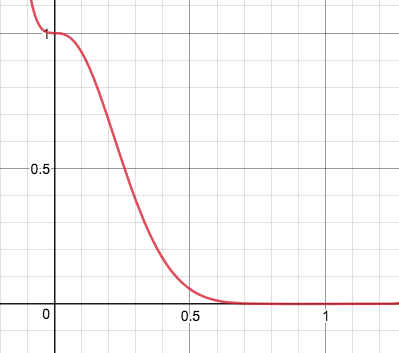
\includegraphics[scale=0.3]{901}
        \end{center}
        The graph above represent the operating characteristic curve with y Axis representing the probability for success and x Axis representing the value of p which is only possible in [0,1]
        \item What happens if we require at most one defective item to accept the
        shipment? Is that a better way to test?
        \begin{center}
        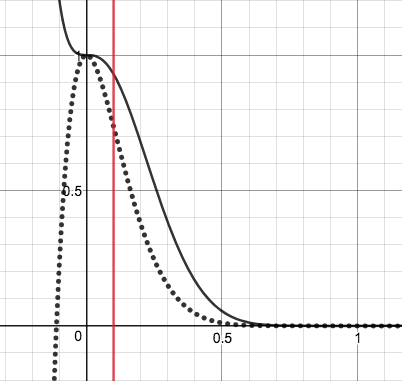
\includegraphics[scale=0.3]{903}
        \end{center}
        The graph above represents the operating characteristic curve with same axis as above. The solid curve represents allowing two defective items out of 10 samples, the dotted curve represents allowing only one defective item out of 10 samples. We want the curve to have as lower acceptance probability as possible when $p\geq 0.1$. As shown in the graph, when $x\geq 0.1$, the dotted curve have fewer acceptance probability than the solid's. Thus only allow one defective item in the sample will effectively prevent the misjudging unacceptable batch as acceptable, thus better in effect. 
        \item What happens if instead of checking 10 items we decide to check 15?
        (We still reject only if there are more than two defective items.) Is that
        a better way to test?
        
        Using the similar method as above: the operating characteristic curve look like this;
        
        \[P(accept)= {15\choose 2}p^2(1-p)^13+{15\choose 1}p(1-p)^14\]
        
        \begin{center}
        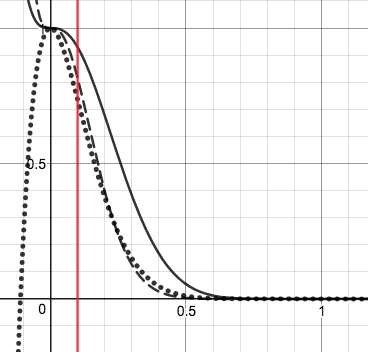
\includegraphics[scale=0.3]{905}
        \end{center}
        
        While the notation remain the same, I added a dashed curve to indicate the new operating characteristic curve. The vertical line represents the equation of $x=0.1$. As shown in the graph, the dashed line have higher acceptance rate when $0\leq p \leq 0.1$. However when $x\geq0.1$, the curve have a higher acceptance rate that the dotted(accept 1 out of 10) and lower acceptance rate than the solid(accept at most 2 out of 10). Thus compare to the solid curve, it is a better way to test. Compare to the dotted line, I would argue it is not a efficient way to test acceptable batch as the curve have a relatively higher acceptance rate even when p surpass 0.1. In this scenario, the objective for a good test curve should be as careful as possible. The dotted curve is  most conservative one and it peaks reasonably around 0.1. Thus it is still the better curve out of 3.
    \end{enumerate}
    
    \item[Problem 10] (2.67) Show that if $X\sim Geom(p)$ then 
    \[P(X=n+k |X>n)=P(X=k) for n,k \geq 1\]
    
    \begin{proof}
    
    $P(X=n+k |X>n)= P(\text{failed at n+1 time, n+2 time, n+3 time... and success at n+k time})$. Since $X\sim Geom(p)$, the events are independent of each other, $P(AB)=P(A)P(B)$. We have:
    \[P(X=n+k |X>n) = \overbrace{P(fail)*P(fail)*...*P(fail)}^\text{k-1 of them}*P(success)= (1-p)^{k-1}p=P(X=k) \]
    \end{proof}
    
    \item[Problem 11] 
    \begin{enumerate}
        \item[3.1]  
        \begin{enumerate}
            \item[(a)] $P(X\leq 3)=1/7+1/14+3/14=3/7$
            \item[(b)] $P(X< 3)=1/7+1/14=3/14$
            \item[(c)] $P(X< 4.12 | X>1.638)=\dfrac{P(X<4.12, X>1.638)}{P(X>1.638)}=2/3$
        \end{enumerate}
        \item[3.2]
        \begin{enumerate}
            \item[(a)] By definition p.m.f must sum to 1: $\sum_{k\in\{1,2,3,4,5,6\}}p(k)= c\sum_{i=1}^6 i= 21c=1$ Thus $c=1/21$.
            \item[(b)] P(X is odd)= P(X=1,3,5)= $\dfrac{1+3+5}{21}=\dfrac{3}{7}$
        \end{enumerate}
        \item[3.4]
        \begin{enumerate}
            \item[(a)] $P(X<6)=\dfrac{2}{6}=\dfrac{1}{3}$
            \item[(b)] $P(|X-7|>1)=P(6<X<8)=\dfrac{2}{6}=\dfrac{1}{3}$
            \item[(c)] $P(X<t | X<6)= \dfrac{P(X<t, X<6)}{P(X<6)}= \dfrac{t-4}{2} $
        \end{enumerate}
    \end{enumerate}
    \end{enumerate}

\end{document}
